\subsection{Outcomes of passive orders}
\label{sec:outcomes}

Each passive order yields one row: its placement time, level, resting size,
volume ahead at placement, the time it reached the front of its queue, and its
end---the first fill, its removal, or the end of observation, whichever came
first. Removal by the owner and censoring by the observation window are kept
apart, as they are different kinds of censoring.

\begin{table}[t]
\centering\small
\caption{Outcomes of passive orders, pilot hour.}
\label{tab:outcomes}
\begin{tabular}{@{}lrr@{}}
\toprule
 & \SOL & \BTC \\
\midrule
Orders & 554\,751 & 1\,743\,849 \\
Fully filled & 0.61\% & 1.39\% \\
Cancelled & 99.11\% & 98.39\% \\
Resting at end of window & 0.28\% & 0.22\% \\
\textbf{At least one fill} & \textbf{0.83\%} & \textbf{1.60\%} \\
\midrule
Median time to first fill & 1.45\,s & 1.43\,s \\
Median time to cancellation & 0.61\,s & 0.42\,s \\
\bottomrule
\end{tabular}
\end{table}

\begin{figure}[t]
\centering
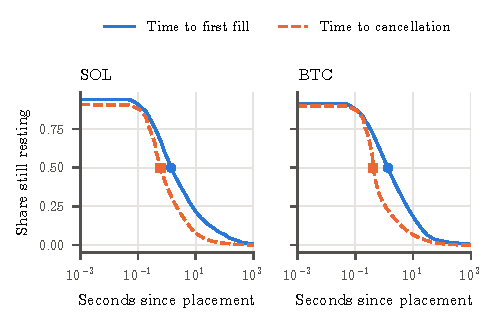
\includegraphics[width=\columnwidth]{lifetimes}
\caption{How long passive orders rest before their first fill (orders that
were filled) and before cancellation (orders that were not), pilot hour. Markers
are medians. Curves start below one because 6--10\% of orders end in the block
in which they were placed.}
\label{fig:lifetimes}
\end{figure}

\paragraph{Cancellation, not non-execution.}
The typical order is withdrawn faster than the typical order is filled
(Table~\ref{tab:outcomes}, Figure~\ref{fig:lifetimes}): 56\% of \SOL{} orders live longer than half a second,
39\% longer than one second, 15\% longer than five. Most orders were not
``unfilled''; they were not observed for long enough to be filled. Treating
cancellation as a negative outcome, as a binary classifier would, charges the
model with errors where the outcome simply did not occur. Fill time is a
survival problem.

\paragraph{Queue position predicts fills monotonically.}
Splitting orders into deciles of volume ahead at placement, the fill rate of
\SOL{} orders falls strictly monotonically from 3.18\% in the first decile to
0.18\% in the last, a seventeen-fold range. Orders joining an empty level fill
three to five times as often as orders joining a non-empty one
(Figure~\ref{fig:deciles}, black).

\paragraph{Strict time priority, verified.}
Of all orders with at least one fill, all but 2 (\SOL) and 32 (\BTC) had
reached the front of their queue no later than their first fill. Each exception
was traced to an order ahead that the exchange removed during matching
(self-trade prevention or a margin cancellation) and that the book stream
records as removed one line after the fill. Time priority thus holds without
exception, and the fill probability factorises:
\begin{equation}
\label{eq:factor}
\Pr(\text{fill}) = \Pr(\text{front}) \cdot \Pr(\text{fill}\mid\text{front}),
\end{equation}
with $6.77\%\times12.26\%=0.83\%$ for \SOL{} and $16.68\%\times9.55\%=1.59\%$ for
\BTC. The factorisation splits fill modelling into two separate questions:
whether an order will reach the front, and whether an aggressor arrives while it
is there. Section~\ref{sec:survival} models both.
